\section{Mise en place de l'infrastructure}
\subsection{Accès ssh à la raspberry pi}
La raspberry pi a été configurée avec l'adresse IP 192.168.1.2. Il faut configurer l'ordinateur avec une adresse IP 192.168.1.x et le masque réseau 255.255.255.0, cela permet aux deux appareils de communiquer.
\subsubsection{Configuration pour VirtualBox}
Pour partager la connexion dans une machine virtuelle, il faut régler le réseau en \textit{Accès par pont} comme le montre l'image ci-dessous.
\begin{figure}[H]
	\begin{center}
		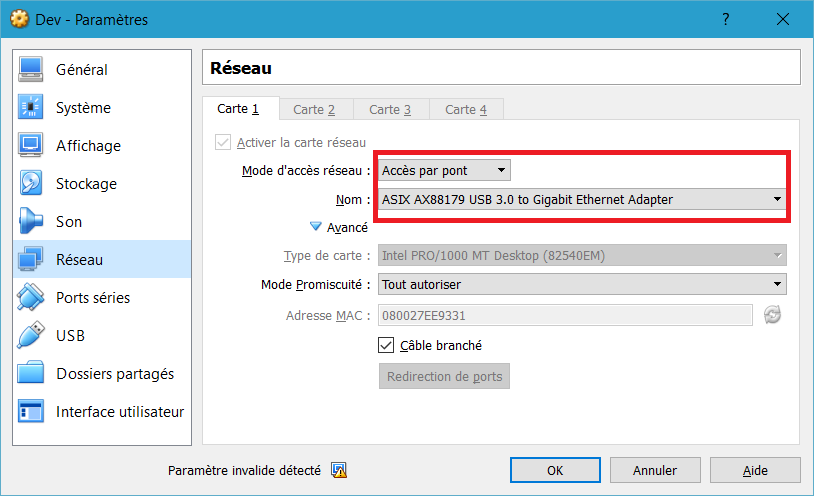
\includegraphics[width=14cm]{img/vmConfig1.png}
		\caption{Configuration de la carte réseau}
		\label{evLinuxConfig1}
	\end{center}
\end{figure}
Il faut également couper la connexion wifi de l'ordinateur, cela lui permettra de se brancher sur la connexion Ethernet.\\
La dernière étape consiste à aller modifier l'adresse IP de la machine virtuelle en changeant les paramètres IPv4. Nous lui avons attribué l'adresse 192.168.1.100.
\begin{figure}[H]
	\begin{center}
		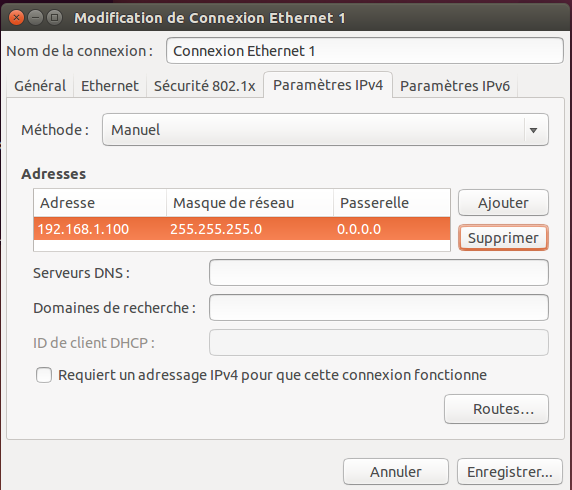
\includegraphics[width=14cm]{img/vmConfig2.png}
		\caption{Changement de l'adresse IP}
		\label{evLinuxConfig2}
	\end{center}
\end{figure}
Il est maitenant possible d'accéder à la raspberry pi par ssh:
\begin{lstlisting}
	$ ssh pi@192.168.1.2
	The authenticity of host '192.168.1.2 (192.168.1.2)' can't be established.
	ECDSA key fingerprint is 80:b2:dc:9d:a5:4e:e7:1a:32:60:11:1c:8b:44:39:0e.
	Are you sure you want to continue connecting (yes/no)? yes
	Warning: Permanently added '192.168.1.2' (ECDSA) to the list of known hosts.
	pi@192.168.1.2's password: 
	...
	pi@raspberrypi:~ $ 
\end{lstlisting}
\subsection{Connexion du capteur}
Pour connecter le capteur à la clé Z-wave, il faut suivre les étapes suivantes:
\begin{enumerate}
	\item Déconnecter le Z-Stick de la Raspberry
	\item Presser le bouton du Z-stick, la LED doit clignoter lentement en bleu
	\item Presser le bouton du capteur
	\item Quand le capteur est inclu/détecter par le Z-Stick, la LED des deux éléments reste figée (vert pour le capteur, bleu pour la clé) quelques instants
	\item Le stick peut ensuite être branché à la Raspberry
\end{enumerate}
\section{Fonctions à implémenter}
Nous devions implémenter les fonctions du groupe 2, soit:
\begin{enumerate}
	\item get\_luminance
	\item get\_motion
	\item get\_battery\_level
	\item get\_all\_measures\_sensors
	\item addNode
	\item removeNode
	\item get\_nodes\\
\end{enumerate}
\textbf{Emplacement du fichier source: }\textit{/backend.py}
\section{REST Client API}
Même si nous n'avions aucune connaissance préalable du REST (discuté lors du premier cours), nous avons tout de même implémenté le client.\\
Nous avons choisi d'utiliser QTCreator et créé une petite application en C++.
\subsection{Lancement de l'application}
\subsubsection{Utilisation de l'exécutable}
L'application a été conçue pour une distribution Linux. Nous avons mis à disposition un exécutable pouvant être lancé de la manière suivante.
\begin{lstlisting}
$ cd executable/
$ ./RESTClient 
\end{lstlisting}
\textbf{Emplacement de l'exécutable: }\textit{/executable/RESTClient}\\\\
La vue par défaut de l'application s'affiche.
\subsection{Utilisation du projet QT}
Nous avons également inclues les sources du projet au cas où l'exécutable ne fonctionnerait pas, ou pour compiler le projet pour un autre environnement que Linux.\\\\
\textbf{Emplacement des sources: }\textit{/RESTClientApp}\\\\
Pour utiliser ces fichiers, il suffit d'installer QT Creator et de double cliquer sur le fichier *.pro des sources, cela va ouvrir le projet. La dernière étape est ensuite de lancer l'application avec le bouton \textit{Run}.
\subsection{Vues de l'application}
Au lancement de l'application, on obtient la vue ci-dessous. La fenêre a été séparée en trois parties distinctes.  La partie centrale va appeler la fonction \textit{get\_all\_measures\_sensors}, tandis que la dernière partie permet de gérer le réseau.\\
Nous avons également inclu un champ permettant de spécifier l'ID du capteur avec lequel on souhaite communiquer.
\begin{figure}[H]
	\begin{center}
		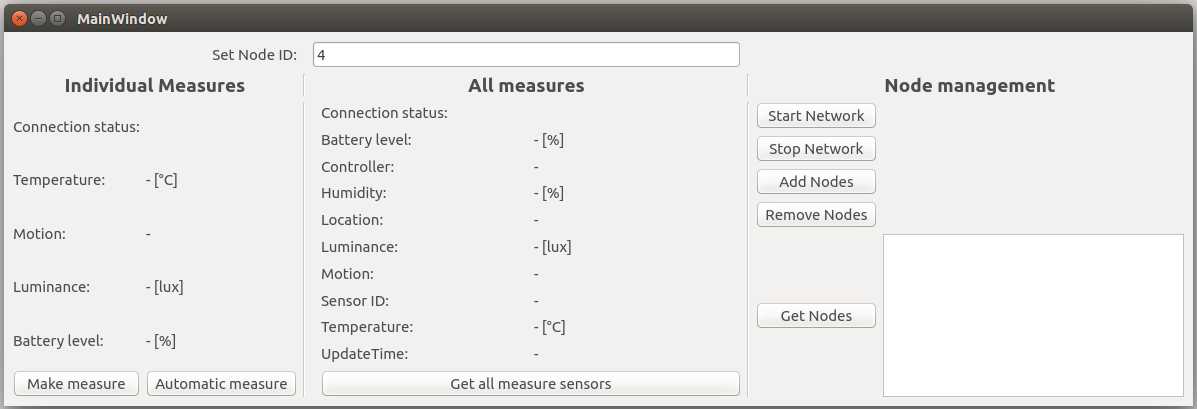
\includegraphics[width=16cm]{img/api1.png}
		\caption{Vue par défaut de l'API}
		\label{api}
	\end{center}
\end{figure}
La première partie de la fenêtre va appeler à la suite les différentes méthodes retournant la température, la luminosité, etc...Elle contient également un bouton enclenchant le mode automatique, les mesures sont répétées toutes les 10secondes, même si nous avons vu que les valeurs se mettent uniquement à jour chaque 10 minutes. Il y a également un champ indiquant le statut de la communication avec le nœud.
\begin{figure}[H]
	\begin{center}
		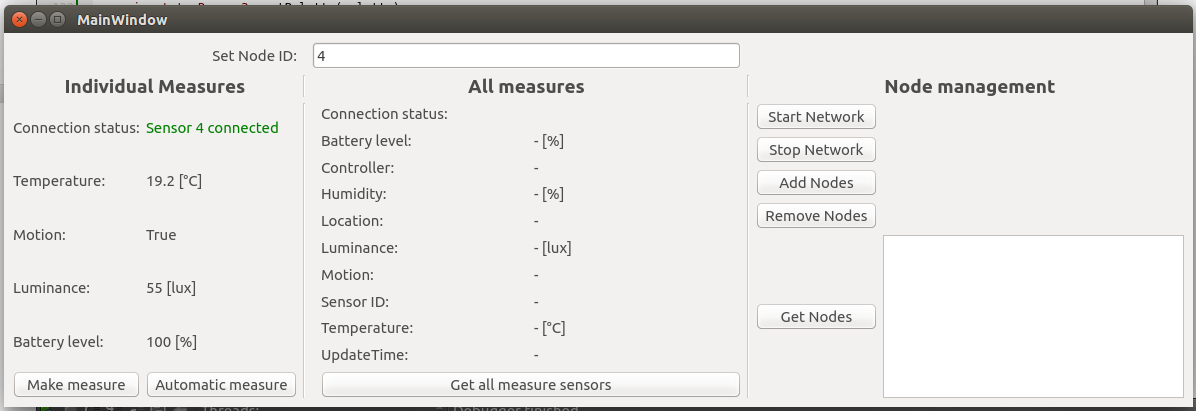
\includegraphics[width=16cm]{img/api2.png}
		\caption{Mesures individuelles}
		\label{api2}
	\end{center}
\end{figure} 

\begin{figure}[H]
	\begin{center}
		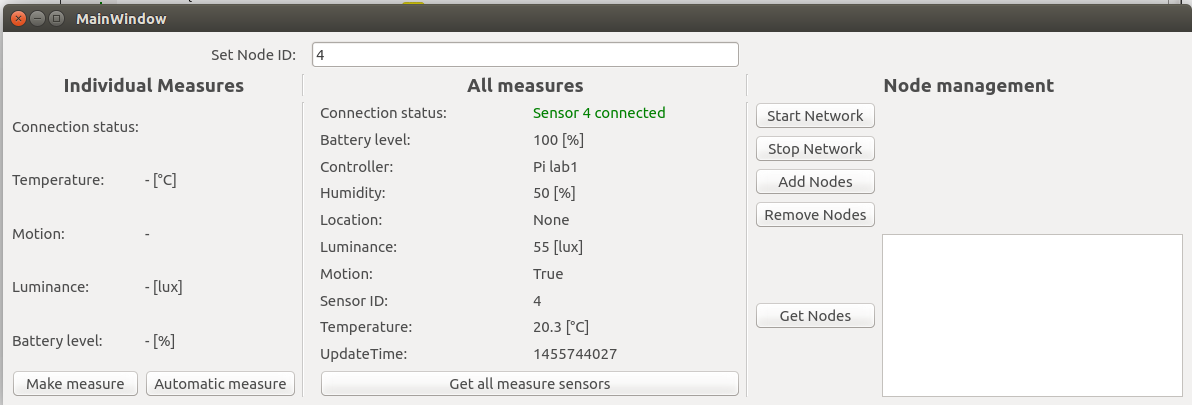
\includegraphics[width=16cm]{img/api3.png}
		\caption{Get all measures}
		\label{api3}
	\end{center}
\end{figure} 
Lorsque l'on appuie sur \textit{Stop network}, le réseau est arrêté et le nœud ne communique plus, un message s'affiche pour informer l'utilisateur.
\begin{figure}[H]
	\begin{center}
		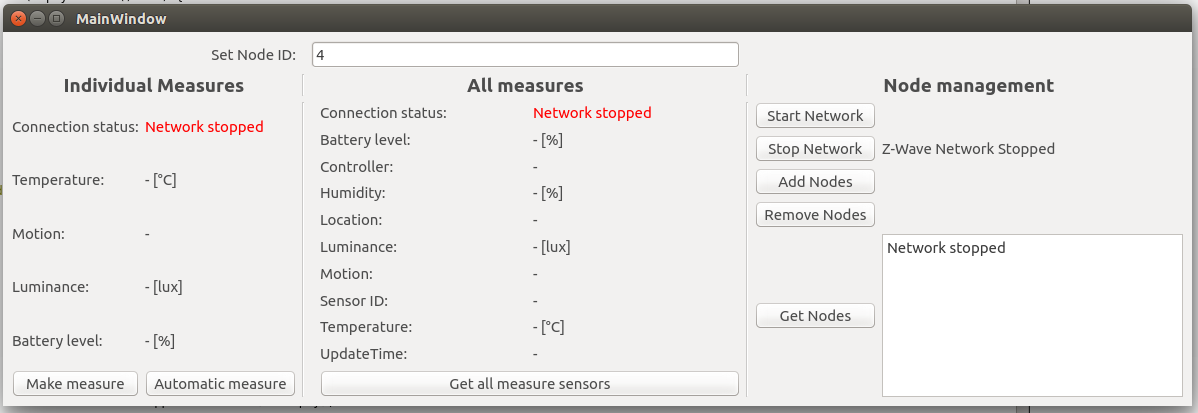
\includegraphics[width=16cm]{img/api4.png}
		\caption{Arrêt du réseau}
		\label{api4}
	\end{center}
\end{figure} 
Le nœud reprend la communication dès que l'on presse \textit{Start network}.
\begin{figure}[H]
	\begin{center}
		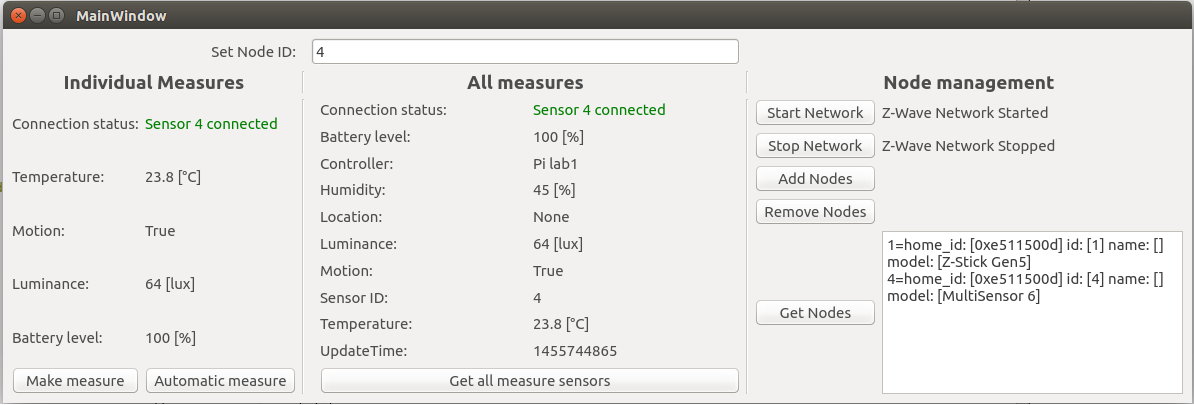
\includegraphics[width=16cm]{img/api5.png}
		\caption{Démarrage du réseau}
		\label{api5}
	\end{center}
\end{figure} 
Pour enlever un noeud du réseau, il faut cliquer sur \textit{Remove node}. Le Z-wave passe en mode exclusion pour 20 secondes. Si l'on appuie sur le bouton du capteur, celui-ci est exclu du réseau. La figure ci-dessous montre ce processus. Le bouton \textit{Get nodes} permet d'afficher à tout instant les nœuds présents dans le réseau.
\begin{figure}[H]
	\begin{center}
		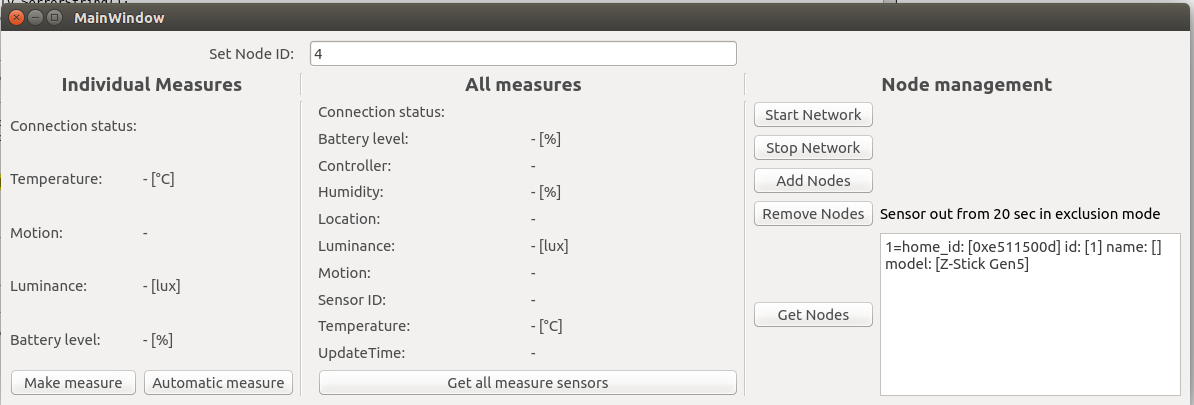
\includegraphics[width=16cm]{img/api6.png}
		\caption{Exclusion du capteur}
		\label{api6}
	\end{center}
\end{figure} 
Le bouton \textit{Add nodes} permet de rajouter un nœud dans le réseau. Le Z-wave passe en mode inclusion pour 20 secondes. Si on appuie sur le bouton du capteur, il rejoindra le réseau. Vu que notre nœud a été précédemment exclu, il est rajouté dans le réseau avec un ID incrémenté de un. Notre capteur a maintenant l'ID 5.
\begin{figure}[H]
	\begin{center}
		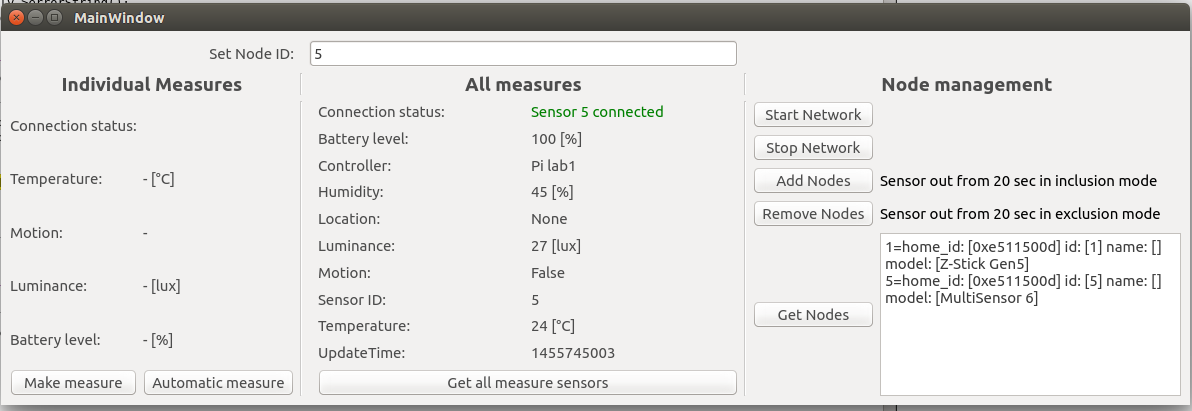
\includegraphics[width=16cm]{img/api7.png}
		\caption{Inclusion du capteur}
		\label{api7}
	\end{center}
\end{figure}